%%=============================================================================
%% EFK
%%=============================================================================

\chapter{EFK}
\label{ch:EFK}

\section{Installatie en configuratie}
Zoals reeds besproken in Hoofdstuk~\ref{subsec:EFK} EFK, bestaat deze stack uit drie belangrijke componenten.
\begin{itemize}
    \item Fluentd
    \item Elasticsearch
    \item Kibana
\end{itemize}
Fluentd is opgebouwd vanuit een push model. Hierbij pusht de service zelf zijn logs naar Fluentd waar ze verwerkt worden. Om deze demonstratie eenvoudiger te tonen wordt hier gebruik gemaakt van dummy logs als input voor Fluentd. Dit zijn standaard logs die geproduceerd worden door een plugin. 
\subsection{Lokale omgeving}
Om de EFK stack lokaal op te zetten wordt vaak gebruik gemaak van compose up. Compose up laat toe om meerdere docker containers tegelijk op te starten. Alle configuratie om de componenten draaiende te krijgen wordt hierin verwerkt. Voor Fluentd wordt binnenin deze compose-up.yaml (zie Listing 5.1) verwezen naar de fluentd.conf file (zie Listing 5.2). In deze .conf file worden de input en output gedefinieerd. In deze configuratie haalt Fluentd logs binnen van verschillende dummy plugins en stuurt deze automatisch door naar een Elasticsearch instantie alsook naar de stdOut. Belangrijk hierbij is de poort van Elasticsearch welke reeds gedefinieëerd werd in de compose-up.yaml (Listing 5.1).

Door simpelweg deze file uit te voeren zullen alle componenten live draaien in hun eigen Docker container. Wanneer dan naar localhost:5601 gekeken wordt kan men de Kibana frontend van deze stack zien. Na het definiëren van een index zullen op de `Discover` pagina  alle logs van deze index terug te vinden zijn. In Figuur 5.1 is het voorbeeld te zien van hoe Kibana eruit ziet met de gebruikte configuratie.

\begin{lstlisting}[caption=Compose up yaml file for EFK]
version: '2'
services:
    fluentd:
        build: ./fluentd
        volumes:
            - ./fluentd/conf:/fluentd/etc
        links:
            - "elasticsearch"
        ports:
            - "8080:8080"
    
    elasticsearch:
        image: docker.elastic.co/elasticsearch/elasticsearch:6.2.4
        environment:
            discovery.type: single-node
        expose:
            - 9200
        ports:
            - "9200:9200"
        
    kibana:
        image: docker.elastic.co/kibana/kibana:6.2.4
        links:
            - "elasticsearch"
        ports:
            - "5601:5601"
\end{lstlisting}

\begin{lstlisting}[caption=Fluentd config file]
<source>
    @type dummy
    dummy {"info":"message 1"}
    tag dummy 1
</source>

<source>
    @type dummy
    dummy {"warning":"message 2"}
    tag dummy 2
</source>

<source>
    @type dummy
    dummy {"error":"message 3"}
    tag dummy 3
</source>

<match **>
    @type copy
    <store>
        @type elasticsearch
        host elasticsearch
        port 9200
        index_name fluentd
        type_name fluentd
        logstash_format true
        logstash_prefix fluentd
        logstash_dateformat %Y%m%d
        include_tag_key true
        tag_key @log_name
        flush_interval 1s
    </store>
    <store>
        @type stdout
    </store>
</match>
\end{lstlisting}

\begin{figure}[ht]
    \centering
    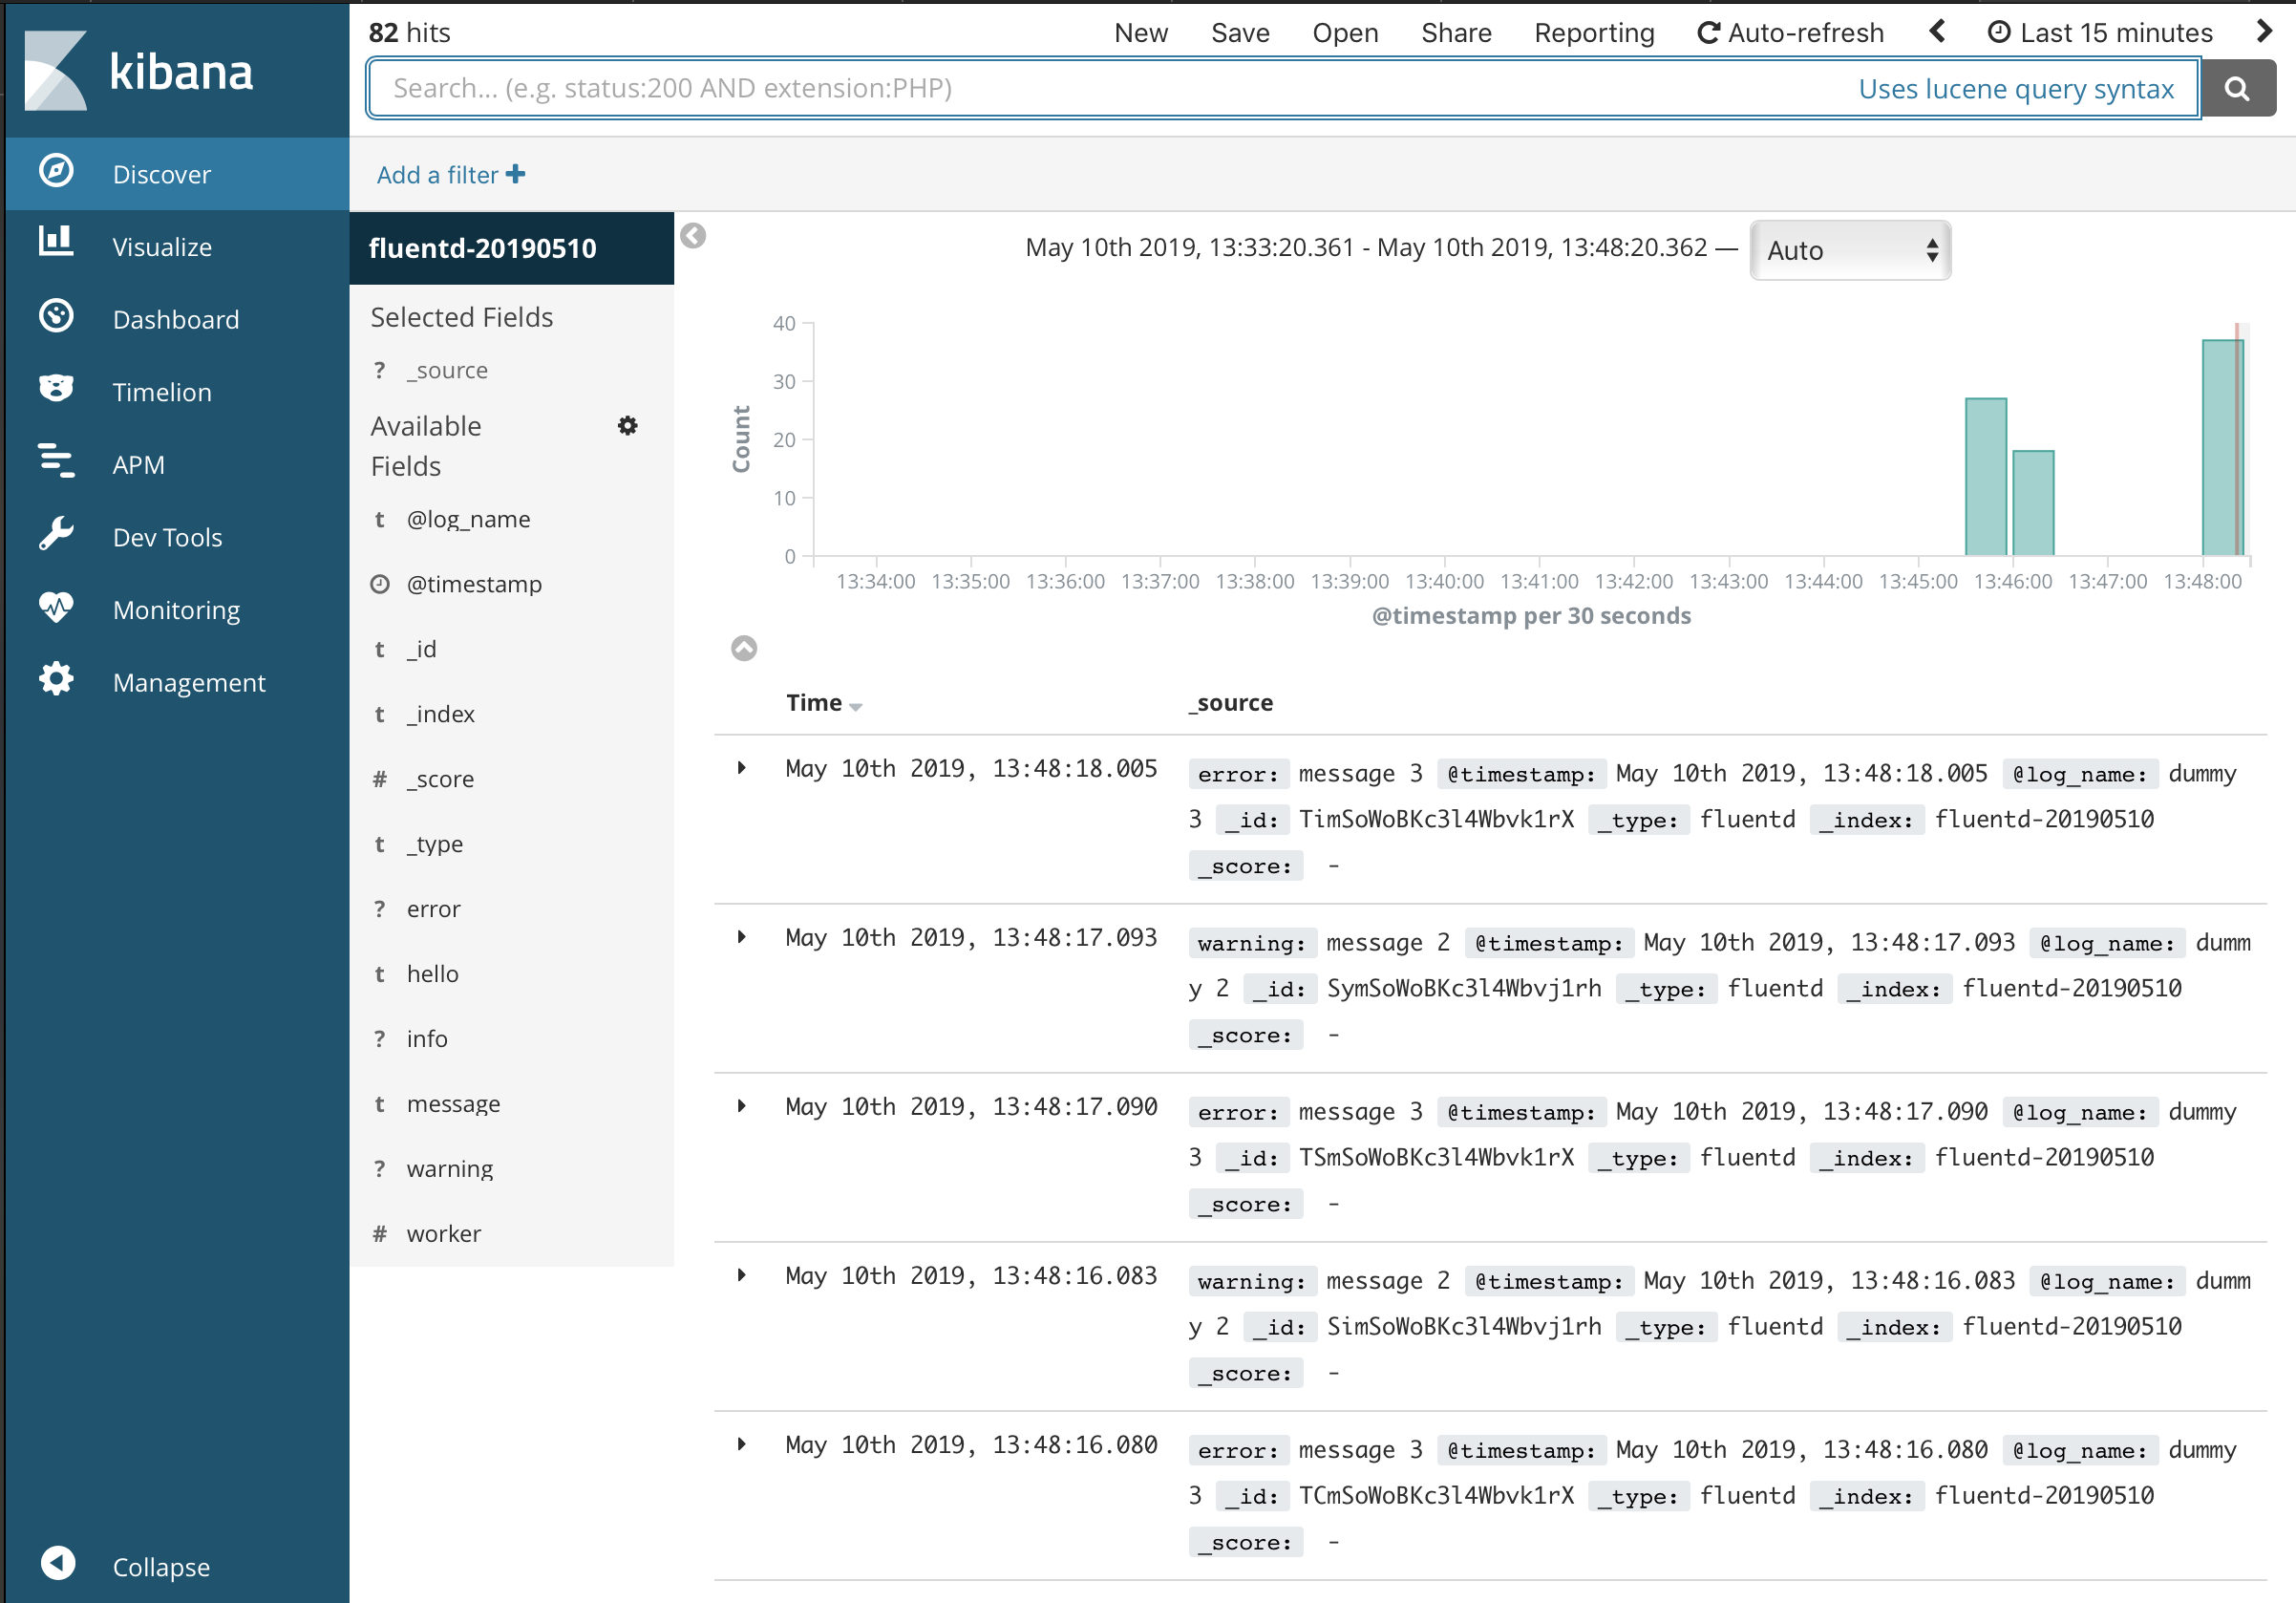
\includegraphics[scale=0.35]{img/EFK-stack}
    \caption[EFK stack frontend]{EFK stack frontend}
\end{figure}

\subsection{Kubernetes omgeving}
De configuratie van de EFK stack voor Kubernetes is ingewikkelder. Hierbij wordt, net zoals bij de ELK stack, gebruik gemaakt van een StatefulSet voor de configuratie van Elasticsearch.

In het artikel van \cite{jetha2018} wordt uitgebreid besproken hoe de EFK stack kan opgezet worden. 

\section{Requirements}

\subsection{Must have}
\subsubsection{Moet open source zijn}
Voor elk van de onderzochte oplossingen geldt dezelfde score voor deze requirement, namelijk 5. Elk van de componenten waaruit een EFK stack bestaat, namelijk Elastischsearch, Fluentd, en Kibana, is vrij te verkrijgen en te gebruiken.

\subsubsection{Ondersteuning voor cluster omgevingen zoals Kubernetes}
Bij de EFK stack geldt een soortgelijke uitleg als bij de ELK of Elastic stack. Dezelfde documentatie welke gebruikt kan worden voor de ELK of elastic stack kan gebruikt worden voor de EFK stack. Met bijkomende documentatie over het configureren van zowel Fluentd als Fluentbit. 

Deze argumenten leiden tot een score van 4 voor de EFK stack.

\subsubsection{Moet een zo klein mogelijke impact hebben op de servers}
Zoals eerder besproken in de sectie~\ref{sec:logging-solutions} heeft deze oplossing een minimale impact op de servers wanneer in acht wordt genomen dat er gebruik wordt gemaakt van Elastiscsearch als databank. Het enige verschilpunt met ELK is dus het gebruik van Fluentd en Fluentbit. Wanneer deze op een correct manier geconfigureerd zijn, zal deze zuiniger zijn op vlak van geheugen gebruik (zie ~\ref{subsec:EFK}, vergelijking tussen Fluentd en Logstash). 

Er blijft wel gebruik gemaakt worden van Elasticsearch waardoor de score voor EFK niet hoger dan 3 kan zijn.

\subsubsection{Moet kunnen scalen naargelang de groeiende Kubernetes cluster}
Ook hier moet gebruik gemaakt worden van een DaemonSet voor de configuratie van Fluentbit om een automatische scaling te garanderen. 

Indien gesteld wordt dat de oorspronkelijke configuratie correct is gebeurd, kan gesteld worden dat de EFK stack automatisch kan scalen naargelang de groei van de cluster. Daarom krijgt EFK een score van 5 voor dit requirement.

\subsection{Should have}
\subsubsection{Moet (relatief) eenvoudig te configureren zijn}
Voor EFK geldt eenzelfde uitleg als de ELK of Elastic stack voor dit requirement. De configuratie van Elastischsearch is ingewikkeld en neemt veel tijd in beslag om correct uit te voeren. 

Fluentd en Fluentbit zijn relatief eenvoudig te configureren en vormen geen probleem voor deze requirement. Wel moet vermeld worden dat de configuratie van Fluentd en Fluentbit moeilijker is dan deze van Logstash en Filebeat \autocite{harikumar2018}.

Om deze redenen krijgt EFK, net als de ELK of Elastic stack, een 2 voor dit requirement.

\subsubsection{Moet (relatief) eenvoudig te gebruiken zijn}
Voor EFK geldt eenzelfde uitleg als de ELK of Elastic stack voor dit requirement. Er geldt een hoge leercurve voor Elasticsearch maar wanneer er sprake is van basis use cases zoals simpele log visualatie in de vorm van simpele grafieken, zal het gebruik van Kibana vanzelfsprekend zijn.

Om deze redenen krijgt EFK, net als de ELK of Elastic stack, een 4 voor dit requirement.

\subsubsection{Moet goed gedocumenteerd zijn}
Voor EFK geldt eenzelfde uitleg als de ELK of Elastic stack voor dit requirement. De Elasticsearch documentatie is zeer uitgebreid. De documentatie van Fluentd en Fluentbit is ook talrijk aanwezig in verschillende officiele en community bronnen.

Voor dit requirement krijgt EFK net als de EFK of Elastic stack een score van 4.

\subsubsection{Moet de logs overzichtelijk kunnen tonen}
Voor EFK geldt eenzelfde uitleg als de ELK of Elastic stack voor dit requirement. De frontend voor de EFK stack is Kibana. De EFK stack beschikt over dezelfde voordelen als de ELK of Elasticstack.

Om deze reden krijgt EFK dezelfde score als de ELK of Elastic stack, namelijk 5.

\subsubsection{Ondersteuning voor verschillende plugins die data extra kunnen verwerken of naar meerdere locaties kunnen doorsturen}
Bij de EFK stack wordt gebruik gemaakt van Fluentbit om de logs te verzamelen en door te sturen naar Fluentd. Deze verwerkt de logs en stuurt deze door naar Elasticsearch. Zowel Fluentbit als Fluentd beschikken over een groot aantal plugins om data te verwerken en door te sturen naar meerdere locaties.

Voor de requirement krijgt de EFK stack een score van 5.

\subsubsection{Ondersteuning voor visualisatie zoals grafieken}
Voor EFK geldt eenzelfde uitleg als de ELK of Elastic stack voor dit requirement. Door het gebruik van Kibana kan gesteld worden dat EFK een uitstekende visualisatie heeft voor alle logs.

Voor de requirement krijgt de EFK stack een score van 5.

\subsection{Could have}
\subsubsection{Ondersteuning voor alerts}
Voor EFK geldt eenzelfde uitleg als de ELK of Elastic stack voor dit requirement. Dankzij Kibana voorziet de EFK stack ondersteuning voor alerts. Deze kunnen via verschillende kanalen verzonden worden.

Voor de requirement krijgt de EFK stack een score van 5.

\section{Resultaten}

Zoals te zien is in tabel~\ref{tab:EFK-resultaten}, scoort EFK een hoge score. Het scoort goed bij de Must Haves en kan dus als een geschikte oplossing beschouwd worden. Het laagste cijfer is een 2, wat gegeven is voor de requirement `Moet (relatief) eenvoudig te configureren zijn`, dit is te wijten aan de complexiteit die gepaard gaat met Elasticsearch. Het scoort de maximale score op verschillende requirements, dit is vooral te wijten aan het gebruik van Kibana.

Een uitgebreide conclusie is te vinden in Hoofdstuk~\ref{ch:conclusie} Conclusie.

\begin{table}[ht]
    \begin{tabular}{| m{20em} | m{2cm} | m{2cm} | m{2cm} | }
        \hline
        \textbf{Requirement}                                                                                              & \textbf{Score (op 5)} & \textbf{Multiplier} & \textbf{Score met multiplier} \\ \hline
        Moet open source zijn                                                                                             & 5                     & 10                  & 50                            \\ \hline
        Ondersteuning voor cluster omgevingen zoals Kubernetes                                                            & 4                     & 10                  & 40                            \\ \hline
        Moet een zo klein mogelijke impact hebben op de servers                                                           & 3                     & 10                  & 30                            \\ \hline
        Moet kunnen scalen naargelang de groeiende Kubernetes cluster                                                     & 5                     & 10                  & 50                            \\ \hline
        Moet (relatief) eenvoudig te configureren zijn                                                                    & 2                     & 5                   & 10                            \\ \hline
        Moet (relatief) eenvoudig te gebruiken zijn                                                                       & 4                     & 5                   & 20                            \\ \hline
        Moet goed gedocumenteerd zijn                                                                                     & 4                     & 5                   & 20                            \\ \hline
        Moet de logs overzichtelijk kunnen tonen                                                                          & 5                     & 5                   & 25                            \\ \hline
        Ondersteuning voor verschillende plugins die data extra kunnen verwerken of naar meerdere locaties kan doorsturen & 5                     & 5                   & 25                            \\ \hline
        Ondersteuning voor visualisatie zoals grafieken                                                                   & 5                     & 5                   & 25                            \\ \hline
        Ondersteuning voor alerts                                                                                         & 5                     & 1                   & 5                             \\ \hline
        \textbf{Totale score}                                                                                             & 47                    &                     & 300                           \\ \hline
    \end{tabular}
    \caption{EFK resultaten}
    \label{tab:EFK-resultaten}
\end{table}